\chapter{Maxwell equations in vacuum}


\newpage
\begin{figure}[H]
\centering
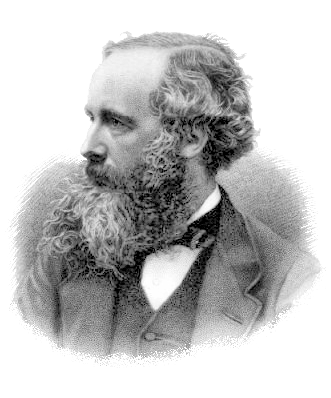
\includegraphics[scale=.3]{src/images/lbk-graphics/portraits/maxwell-wiki.png}
\caption*{}
\end{figure}
%~ \portrait{.4}{lbk-graphics/portraits/maxwell-wiki.png}

\begin{quote}Engraving of James Clerk
Maxwell by  G. J. Stodart from a photograph by Fergus of
ngGreenockl
\end{quote}


\begin{small}
\begin{quote}

James Clerk Maxwell FRS FRSE (13 June 1831--5 November 1879) 
was a Scottish  scientist in the field of mathematical 
physics.  His most notable achievement was to formulate the 
classical theory of electromagnetic radiation, bringing 
together for the first time electricity, magnetism, and 
light as manifestations of the same phenomenon.  Maxwell's 
equations for electromagnetism have   been called the 
"second great unification in   physics"  after the first one 
realised by Isaac Newton.

His discoveries helped usher in the era of modern physics, 
laying the foundation for such fields as special relativity 
and quantum mechanics. Many physicists regard Maxwell as 
the  19th-century  scientist having the greatest 
influence on  20th-century physics. His contributions to 
the  science are considered by many to be of the same 
magnitude as those of Isaac Newton and Albert Einstein. In 
the millennium poll--a survey of the 100 most prominent 
physicists--Maxwell was  voted the third greatest 
physicist of all time, behind only Newton and Einstein. On 
the centenary of Maxwell's birthday, Einstein described  
Maxwell's work as the "most profound and the  most 
fruitful that physics has experienced since  the time of 
Newton".\hfill-Wikipedia
\end{quote}
\end{small}

%%%%%%%%%%%%%%%
\newpage



\section{Introduction}
Here, we learn that the familiar (3-vector) Maxwell-   
Lorentz equations in vacuum are actually a pair of    
4-tensor equations. The crucial input in this exercise is 
the fact that {electric charge is a Lorentz invariant}. 
This fact which is amply supported by experiments implies 
that the 3-scalar charge-density $\rho$ and the  3-vector  
current-density $ \vec{J} \equiv \rho\vec{u}$ together form 
a 4-vector called the \textsl{charge-current-density 
4-vector}. Before discussing  that, we do a quick review of 
the Maxwell equations in the 3-vector format.

In an inertial frame S, we consider an electromagnetic  
field, \textsl{in vacuum}, described by the familiar pair 
of  3-vectors $\{\vec{E}(\vec{r}, t), 
\vec{B}\break (\vec{r}, t)\}$. These 3-vector fields,  in vacuum, 
are due to \textsl{distributed sources} characterized by a 
\textsl{charge-density} $\rho = \rho(\vec{r}, t)$ and a 
\textsl{3-vector current-density}  $\vec{J} \equiv 
\vec{J}(r, t) = \rho(\vec{r}, t)\vec{u}(\vec{r}, t) $,  and 
evolve in  space and time as governed by the 
\index{Maxwell-Lorentz equations in vacuum} 
\textsl{Maxwell-Lorentz} equations\footnote{We use the SI 
units.} 
\begin{align}\label{ved.1}
&\vnab \dotp \vec{E} = \rho/\varepsilon_0, \\
&\vnab \dotp \vec{B} = 0, \label{ved.2} \\
&\vnab \cross \vec{E}+(\dow\vec{B}/\dow t)= 
0,\label{ved.3}\\
&\vnab \cross\vec{B} - (1/c^2) (\dow\vec{E}/\dow t)
= \mu_0 \vec{J}.\label{ved.4}
\end{align}
Here, $\varepsilon_0 $ and $ \mu_0 $, respectively called 
the \textsl{vacuum permittivity} and\  \textsl{vacuum 
permeability},  are two universal constants  . They bear 
the relation
\begin{align*}
\varepsilon_0 & = (1/c^2) \mu_0 = \SI{1.3566 e-8}{m\,
kg\,C^{-2}},
\end{align*}
where $c$ is the vacuum velocity of light. The equations 
\eqref{ved.2} and \eqref{ved.3} which do not contain the 
source terms $\rho$ and $\vec{J}$ are called 
\textsl{homogeneous equations} while the other two 
equations 
\eqref{ved.1} and \eqref{ved.4} are called 
\textsl{non-homogeneous equations}. It is now an 
experimentally established fact that \textsl{these 
equations 
are valid in every inertial frame}. By this statement, we 
mean the following: \begin{quote} \textsl{If, in one 
inertial frame $S$, in a certain region $\mathbb{M}_R $ of 
spacetime, these equations \eqref{ved.1}-\eqref{ved.4} hold 
with the  field and source variables
\begin{align*}
\{\vec{E} , \vec{B}, \rho, \vec{J} = \rho\vec{u} \},
\end{align*}
then, in some other inertial frame $S'$, obtained from $S$ 
by a Lorentz transformation, the same equations 
\eqref{ved.1}-\eqref{ved.4} hold in $\mathbb{M}_R$ with 
the  $S$-frame-variables respectively replaced by  
the $S'$-frame-variables
\begin{align*}
\{\pvec{E}, \pvec{B}, \rho', \pvec{J}= \rho'\pvec{u} \}.
\end{align*}}
\end{quote}

\section{The charge-current-density 4-vector}
In an inertial frame $S$ in which a certain tiny 
globule (to be precise, charged matter occupying an 
infinitesimal spatial volume) of charged matter is 
\textbf{at rest}, the charge-density of the globule, 
called its \textsl{proper-charge-density}, is given by
\begin{align}\label{ved.5}
 \rho_0 =(\dd q/ \dd V_0 ),
\end{align}
where $\dd V_0$ is the infinitesimal spatial volume of the 
tiny-globule which has an electric charge $\dd q$.  The 
proper  charge-density $\rho_0$ is  a 
\textsl{Lorentz-scalar} as $\dd q$ and $\dd V_0 $, are so. 

Let us consider the infinitesimal globule in another 
inertial frame $S'$ related to $S$ by an x-boost with 
$\vec{\gkb}=u\,\eye$. In $S'$, the globule would be 
in uniform motion with velocity $-u\,\eye\,'$, and 
would have the same charge $\dd q$, as charge is a 
Lorentz-scalar. If $\rho$ is the charge density and $\dd V= 
\dd x'\dd y'\dd z'$ is the (spatial) volume of the globule 
in the frame $S'$, we must have
\begin{align*}
\rho_0\,\dd V_0&=\dd q= \rho\,\dd V= \rho\,\dd x'\dd y'\dd 
z'=\rho\,(\dd x/\Gamma)\dd y\dd z\notag\\& 
=(\rho/\Gamma)\,\dd V_0,
\end{align*}
where $\dd V_0=\dd x\dd y\dd z$, and  we have used the 
results that under the x-boost the length-element $\dd x$ 
has 'Lorentz-contracted' to $\dd x'=(\dd x/\Gamma)$ while 
the length-elements $\dd y$ and $\dd z$ remain unchanged. 
The symbol $\Gamma$ in the equation above 
is the familiar gamma-factor $(1-u^2/c^2)^{-1/2}$ associated 
with the 3-velocity $\vec{u}$ of the charge. Thus, under an  
x-Lorentz-boost  from $S$ to $S'$,  which has a velocity 
$\vec{u}=(u,0,0)$ in $S$,  charge-density transforms by the 
rule
\begin{align}\label{ved.6}
\rho=\Gamma\rho_0.\quad \Gamma&\equiv 
\frac{1}{\sqrt{1-u^2/c^2}},
\end{align}
Here, $\rho$ is the charge-density of the globule in the 
frame $S'$ in which it is in motion with the velocity 
$\vec{u}=(u,0,0)$, and is called its \textsl{relative 
charge-density}.

Next, multiplying $\rho$ and $\vec{u}$, we obtain the 
\textsl{3-current-density} vector field associated with the 
charged globule in $S'$ : 
\begin{align}\label{ved.7}
\vec{J}=\rho\vec{u}=\Gamma \rho_0=\frac{\rho_0\vec{u}}
{\sqrt{1-u^2/c^2}},
\end{align}
which, incidentally, shows that the 3-current-density vector 
vanishes in  the rest-frame $S$ of the charged globule.

When combined, the 3-charge-density $\rho$ and the 
3-current-density  $\vec{J}=\rho \vec{u}$ in a given 
inertial frame, such as the frame $S'$ considered 
above, yield a 4-vector:
\begin{align}\tag{8.8a}
( c\rho, \vec{J})=\rho( c, \vec{u}) = \Gamma \rho_0
( c, \vec{u}),
\end{align}
where we may recall that  $U^\gka =\Gamma ( c, \vec{u})$ is 
the 4-velocity of the infinitesimal globile in $S$.  From 
Eqn.(8.8a), we thus identify a 4-vector $J^\gka$ with 
the contravariant-components 
\begin{align}\label{ved.8}
J^\gka \equiv \rho_0 U^\gka 
= \rho_0\Gamma\sdv{x^\gka}{t}=\rho\sdv{x^\gka}{t}
=( c\rho, \vec{J}),
\end{align}
which is called the called the 
\textsl{charge-current-density 4-vector}. It is useful to 
note that the charge-current-density 4-vector has the 
covariant components 
\begin{align}\tag{8.8a}
J_\gka =\eta_{\gka \gkb}J^\gkb =( c\rho, -\vec{J}).
\end{align}
\section{The 4-gradient operator}
In what follows, we need to use the 4-gradient operator that
we introduced in \S~5.5.1:
\begin{align}\label{ved.9}
\dow_\gka =\left(\frac{1}{c}\,\frac{\dow}{\dow t}, 
\frac{\dow}{\dow x}, \frac{\dow}{\dow y}, 
\frac{\dow}{\dow z}\right)
=\left(\frac{1}{c}\frac{\dow}{\dow t},\vnab \right).
\end{align}
We may recall that this is a \textsl{covariant} vector 
operator and its  \textsl{contravariant} components are
\begin{align}\label{ved.10}
\dow^\gka =\eta^{\gka \gkb}\dow_\gkb
= \left(\frac{1}{c}\frac{\dow}{\dow t},-\vnab \right).
\end{align}
\section{Law of conservation of electric charge. The 
equation of continuity}
Recall the familiar statement  "electric charge can neither 
be created nor destroyed". This is the law of conservation 
of charge. It implies that in  a closed system, the amount 
of charge, \ie, the algebraic sum of the positive and 
negative charges of the system, remains the same. The law 
also means that when charges are allowed to be exchanged 
between two systems, say A and B in contact, whatever charge 
is lost by, say, A,  must have been  transfered to B. In 
classical electrodynamics, we model electric charge as a 
continuous distribution: As such, one introduces the 
concepts  of the 'flow of charges' (both positive and 
negative), charge density,  currents (of charges) and 
current density to deal with such a continuum of charge. 
This, in turn, requires that the law of conservation of 
charge is also formulated appropriately. 

In the infinitesimal neighbourhood of a point in a 
continuous distribution of charge in vacuum, the law of 
conservation of electric charge may be expressed as the  
following differential equation
\begin{align}\label{ved.11x}
0&=\pdv{\rho}{t} +\vnab \dotp\vec{J},
\end{align}
called the equation of continuity. Equation \eqref{ved.11x} 
describes the law of  conservation of electric charge in the 
'differential neighbourhood' of a point in a continuum of 
charge and  is called a  'local law' for this reason. In 
contrast, later we also express the law  as an integral 
equation which holds over a region in the charged 
continuum. 

First, we obtain the local (or differential) form of the law 
which follows from the  Maxwell equations  \eqref{ved.1} to 
\eqref{ved.4}: On taking the divergence of 
Eqn.\eqref{ved.4}, we obtain
\begin{align*}
\vnab\dotp(\vnab\cross\vec{B})-(1/c^2)(\dow/\dow
t)(\vnab\dotp\vec{E})=\gkm_0\vnab\dotp\vec{J},
\end{align*}
where we have swapped\footnote{The operators $\dow/\dow t$, 
$\dow/\dow x$, $\dow/\dow y$, $\dow/\dow z$, being 
derivative operators with respect to independent coordinates 
$t$, $x$, $y$, $z$, all commute with one another.} the 
commuting operators $(\vnab\dotp)$ and  $(\dow/\dow t)$ in 
the second term on the left hand side. Now substituting for 
$\vnab\dotp\vec{E}$ in the above equation from  
Eqn.\eqref{ved.1} and using $\vnab\cross\vec{B}=0$ from 
Eqn.\eqref{ved.2}, we get
\begin{align*}
-(1/c^2\epso)\pdv{\gkr}{t}
=\gkm_0\vnab\dotp\vec{J}.
\end{align*}
If we use relation $\epso\gkm_0=1/c^2$ and rearrange this 
equation, we get the equation of continuity 
Eqn.\eqref{ved.11x} which is the mathematical statement of 
the \textsl{local law of conservation of charge}.

\begin{figure}[H]
\begin{center}
\begin{tikzpicture}
%   \draw[help lines,step=.25,red] (-2,-2) grid (2,2) ;
%   \foreach \y in {-2,-1.5,...,2}
%     \draw (-2.2,\y) node[left]{\tiny\y} ;
%   \foreach \x in {-2,-1.5,...,2}
%     \draw (\x,-2.2) node[below]{\tiny\x} ;
\node at (0,0)
{\includegraphics[scale=.7]%
{src/images/lbk-graphics/region-omega-bw}};
\node at (0,.5){\scriptsize continuous charge}; 
\node at (0,.2){\scriptsize distribution};
\node at (-1,-.15){\small $V$};
\node at (1.25,-.6) {$\sigma$};
\node at (.2,-1.35) {$\hat{n}$};
\end{tikzpicture}
\end{center}
\caption{Region of integeration} 
\label{8.1}
\end{figure}

As already remarked, the equation of continuity 
\eqref{ved.11x} may also be expressed in an  
\textsl{integral form} as follows: Let $\gks$ be an 
arbitrary,  fixed\lbk (\ie, unchanging),  \textsl{simple 
closed-2-surface} (see \figref{8.1}) and let $V$ be the 
3-dimensional spatial region enclosed $\gks$. Integrating 
Eqn.\eqref{ved.11x} over $V$, we get
\begin{align}\label{ved.12x}
\int_V \vnab\dotp\vec{J}\,\dd V
=- \int_{_V} \nt\frac{\dow\gkr}{\dow t}\,\dd 
V=-\frac{\dow}{\dow t} \nt\int_{_V} 
\nnt\gkr\,\dd V,
\end{align}
where, in the last term on the right hand side, we have 
pulled the operator $(\dow/\dow t)$ out of the integral sign 
as the region of integration $V$ is fixed and unchanging in 
time. But, $\int_{_V}  \gkr\,\dd V$ is  the total 
electric charge $Q$ contained in $V$.  Thus, 
Eqn.\eqref{ved.12x} becomes
\begin{align*}
\int_{_V}\vnab\dotp\vec{J}\,\dd V=-\pdv{Q}{t}.
% =-\oint_\gks (\dow\gkr/\dow t)\,\hat{n}\,\dd \gks ,
\end{align*}
Finally, using the Gauss theorem, we convert the volume 
integral  $\int_{_V} \vnab\dotp\vec{J}\,\dd V$ 
above into an integral over the simple closed-2-surface 
$\gks$ which encloses $V$ and rewrite the above equation  
as
\begin{align}\label{ved.13x}
\oint_\gks (\vec{J}\dotp \hat{n})\,\dd \gks=-\frac{\dow 
Q}{\dow t}\,.
\end{align}
Here, $\hat{n}$ is the out-ward-drawn normal to the simple 
closed-2-surface $\gks$. This equation \eqref{ved.13x} is 
the  mathematical statement of the fact that the amount of 
electric charge that flows out of the simple 
closed-2-surface $\gks$ in unit time is equal to the 
decrease, per unit time, of the net electric charge enclosed 
by the surface $\gks$. 

In passing, we note that Eqn.\eqref{ved.13x} and 
\eqref{ved.11x} both describe the law of conservation of 
electric charge mathematically: However, 
Eqn.\eqref{ved.13x} holds for the finite region $V$ enclosed 
by $\gks$ while \eqref{ved.11x}  is a local law true in the 
neighbourhood of a point. 

\hbf{The covariant-form of the equation of continuity}
Lastly, we observe that the continuity  equation 
Eqn.\eqref{ved.11x} may also be rewritten as
\begin{align}\label{ved.14x}
0&=\frac{\dow(c\rho)}{\dow (ct)}+\frac{\dow J_x}{\dow x}
+\frac{\dow J_y}{\dow y}+\frac{\dow J_z}{\dow z}
\notag\\
&=\dow_0 (c\rho) +\sum_{k=1}^3 \dow_k J^k= \dow_\gka 
J^\gka ,
\end{align}
which is clearly, a tensor  equation (also referred to 
as a covariant equation). 
We may state this equation verbally as ``\textsl{the 
4-divergence of the 4-current density is identically 
zero}''.

\vspace{-.2cm}

\section{Electromagnetic potentials}
Observe that the vacuum Maxwell equation $\vnab \dotp 
\vec{B}=0$ is automatically satisfied by a
vector function of the form
\begin{align*}
\vec{B}(t,\vec{r})= \vnab \cross \vec{A}(t,\vec{r}),
\end{align*}
where $\vec{A}\equiv \vec{A}(t,\vec{r}) $ is {any} smooth 
function of its arguments. If we replace $\vec{B}$ by $\vnab 
\cross \vec{A}(t,\vec{r})$ in the Maxwell equation 
\eqref{ved.3}, we get
\begin{align*}
0=\vnab \cross \vec{E}+\frac{\dow}{\dow t} 
(\vnab \cross\vec{A}) =\vnab \cross \left(\vec{E} + 
\frac{\dow\vec{A}}{\dow t} \right).
\end{align*}
This shows that the terms in the brackets in the last term 
on the right is the gradient of {any} differentiable, 
3-scalar function of ($t,\vec{r}$), say, $\phi(t,\vec{r})$, 
\ie,
 \begin{align*}
\vec{E}+ \pdv{\vec{A}}{t}=-\vnab \phi.
\end{align*}
Thus, two of the vacuum Maxwell equations, namely, the 
source-term-free equations  \eqref{ved.2} and \eqref{ved.3}, 
are automatically satisfied if the electric and magnetic 
fields $(\vec{E}, \vec{B})$ are determined in terms of the 
functions $\phi(t,\vec{r} ), \vec{A}( t,\vec{r}))$ as 
given by the  equations
\begin{align}\label{ved.15x}
&\vec{E}= -\vnab \phi- \frac{\dow\vec{A}}{\dow t}, 
\\\label{ved.16x}
&\vec{B}= \vnab \cross \vec{A}.
\end{align}
The two functions $\phi (t,\vec{r})$ and 
$\vec{A}(t,\vec{r})$, here,  are called the \textsl{scalar 
and  vector potentials} of the vacuum electromagnetic field.

At the moment, the scalar and  vector potentials, $\phi 
(t,\vec{r})$ and $\vec{A}(t,\vec{r})$, which define
the vector fields $\vec{E}$ and $\vec{B}$,  are completely 
arbitrary except for the  requirements of differentiability. 
The fields $\vec{E}$ and $\vec{B}$ obtained from  
the potentials, through the equations 
\eqref{ved.15x} \eqref{ved.16x} satisfy only two of the four
Maxwell equations: To be a physically acceptable set of 
field vectors,  they must also satisfy  
the remaining two vacuum Maxwell equations, namely, the 
equations \eqref{ved.1} and \eqref{ved.4}.  

To check whether this is true, first we plug the fields 
$\vec{E}$ and $\vec{B}$ obtained from \eqref{ved.15x} and 
\eqref{ved.16x} into \eqref{ved.4} and obtain
\begin{align*}
\mu_0 \vec{J} &=\vnab \cross \vec{B}- \mu_0\eps_0 \frac{\dow 
\vec{E}}{\dow t}\\
&=\vnab \cross(\vnab \cross \vec{A}) - \frac{1}{c^2} 
\frac{\dow }{\dow t}\bigg(-\vnab \phi- \frac{\dow \vec{A}} 
{\dow t}\bigg).
\end{align*}
Here, on the right hand side, we use the well known 
differential-vector-identity 
\begin{align*}
 \vnab \cross(\vnab\cross \vec{A})=\vnab \left(\vnab \dotp 
\vec{A} \right)-\nabla^2\vec{A}, 
\end{align*}
to rewrite the first term and also  swap the partial 
differential operators $\vnab$ and $\pdv{}{t}$ in the third 
term. This changes give  
\begin{align}\tag{8.17a}
\mu_0 \vec{J}
&= \vnab \left(\vnab \dotp \vec{A} \right)
-\nabla^2\vec{A} +\frac{1}{c^2}\vnab \left(
\frac{\dow\phi}{\dow t}\right)+\frac{1}{c^2}
\frac{\dow^2\vec{A}}{\dow t^2}.
\end{align}
Changing the sign throughout, we  rearrange this  
equation as
\begin{align}\label{ved.17x}
\Box\vec{A}- \vnab {\lambda}= -\mu_0\vec{J},
\end{align}
where
\begin{align}\label{ved.18x}
\lambda \equiv \vnab \dotp \vec{A}+\frac{1}{c^2}
\frac{\dow\phi}{\dow t},
\end{align}
and the 'box-operator' $\Box$  is the familiar 
\textsl{d'Alembertian operator}
\begin{align}\label{ved.19x}
\Box \equiv \nabla^2 -\frac{1}{c^2}\frac{\dow^2}{\dow t^2},
\end{align}
which is also called the \textsl{wave-operator} in 
3-dimensions. 

Next, we plug the potentials $\phi$ and $\vec{A}$ defined in 
Eqns. \eqref{ved.15x} and \eqref{ved.16x} into 
Eqn.\eqref{ved.1} and obtain, on using the function 
$\lambda$ defined in Eqn.\eqref{ved.17x},
\begin{align*}
\frac{\rho}{\epso}
&=\vnab \dotp \bigg( -\vnab \phi- \frac{\dow\vec{A}}{\dow
t}\bigg)=-\nabla^2\phi- \frac{\dow}{\dow t} (\vnab \dotp
\vec{A})
\\&=-\nabla^2\phi-\frac{\dow}{\dow t} \left(\lambda 
-\frac{1}{c^2}\frac{\dow\phi}{\dow t}\right)  
=-\nabla^2\phi+\frac{1}{c^2}\frac{\dow^2\phi}{ \dow t^2} 
-\frac{\dow\lambda}{\dow t},
\end{align*}
Using the d'Alembertian operator, we rearrange this 
equation as
\begin{align}\label{ved.20x}
\Box \phi+\frac{\dow\lambda}{\dow t}= -\frac{\rho}{\epso}.
\end{align}
The equations \eqref{ved.17x} and 
\eqref{ved.20x}, with the function $\lambda$ is defined in 
 Eqn.\eqref{ved.18x},  determine the vacuum  Maxwell field 
$(\vec{E},\vec{B})$ in terms of the scalar and vector 
potentials $(\phi,\vec{A})$.

However, the potential-form of the vacuum Maxwell  
equations have a \textsl{blind spot}. While a given pair of  
 potentials $(\phi,\vec{A})$ determine the fields 
$(\vec{E},\vec{B})$ uniquely   through \eqref{ved.15x} and 
\eqref{ved.16x}, the converse is not true: {As we shall see 
in the following paragraphs, there exists a whole family of 
potentials $\{(\phi,\vec{A})\}$, each of which gives rise 
to the same Maxwell fields $(\vec{E},\vec{B})$} through 
equations \eqref{ved.15x} and \eqref{ved.16x}.

\subsection{Gauge transformations}
Let $\gkc(t, \vec{r}) $ be an arbitrary differentiable 
function of its  arguments. With such a function $\gkc$, 
let us define a new vector potential $\pvec{A}$ by
\begin{align}\label{ved.21x}
\pvec{A} =\vec{A}+ \vnab \gkc .
\end{align}
Then, as $\vnab \cross(\vnab \gkc ) $ is identically zero, 
$\vnab\cross\pvec{A}=\vnab\cross\vec{A}=\vec{B}$ which shows 
that every member of an entire family of 3-vector potentials 
$\pvec{A}$ defined by Eqn.\eqref{ved.21x} gives rise to the 
same magnetic 3-vector $\vec{B}$. However, although 
$\vec{B}$ is unchanged when $\vec{A}\mapsto \pvec{A} $ 
through Eqn.\eqref{ved.21x}, the electric 3-vector $\vec{E}$ 
does not remain the same. It changes to
\begin{align}\label{ved.22x}
\vec{E} &= -\vnab \varphi-(\dow \vec{A}/\dow t)=-\vnab 
\varphi -(\dow /\dow t) (\pvec{A}-\vnab \gkc ) \notag 
\\&=-\vnab (\varphi-\dow \gkc /\dow t) - (\dow 
\pvec{A}/\dow t).
\end{align}
Therefore, in order to keep $\vec{E}$ also unchanged when  
$\vec{A}\mapsto \pvec{A}$ through Eqn.\eqref{ved.21x}, we 
must simultaneously  change the scalar  potential from 
$\varphi $ to a new scalar  potential $\varphi'$ given by
\begin{align}\label{ved.23x}
 \varphi'= \varphi-\dow \gkc /\dow t.
\end{align}
Thus, we observe that the fields $\{\vec{E},\vec{B}\}$ do 
not change if we replace the potentials $\{\varphi, 
\vec{A}\}$ to $\{\varphi', \pvec{A}\}$ as specified in the 
equations \eqref{ved.21x} and \eqref{ved.23x}. The  
equations \eqref{ved.21x} and \eqref{ved.23x} are called  
\textsl{gauge (scale) transformations of the  
electromagnetic potentials}. Such a gauge  transformation is 
generated by a single, arbitrary, scalar function $\gkc 
(t,\vec{r})$ which is called the \textsl{generator} of the 
gauge transformation.

Suppose we have a vacuum electromagnetic field  which is 
described by a generic pair of potentials $\{\varphi, 
\vec{A}\}$ satisfying the equations \eqref{ved.17x} and 
\eqref{ved.20x}. Let us perform a a gauge 
transformation  of $\{\varphi, \vec{A}\}$ with a 
generator $\gkc$ and obtain the gauge transformed 
potentials $\{\varphi', \pvec{A}\}$. One can 
show\footnote{See any standard text on classical 
electro-dynamics such as Griffiths, loc.cit.} that 
by choosing  $\gkc$ appropriately, the gauge 
transformed potentials ${\varphi', \pvec{A}}$ satisfy 
one of the following, much used, convenient conditions, 
namely,
\begin{align}\label{ved.24x}
 \lambda' \equiv \vnab \dotp \pvec{A}+\frac{1}{c^2}
\frac{\dow\phi'}{\dow t}=0,
\end{align}
called the \textsl{Lorenz\footnote{This gauge is often 
erroneously attributed to the Dutch physicist H. A. Lorentz. 
It was actually published by the Danish physicist L. 
Lorenz.} gauge condition}, or,
\begin{align}\label{ved.25x}
\vnab \dotp \pvec{A}=0,
\end{align}
called the \textsl{Coulomb gauge condition}.

Apart from the above two standard gauge choices for the 
potentials, many other choices are possible which are used 
in electrodynamics\footnote{See for instance, L.D.Landau 
and E.M.Lifshitz, Ref. [1]}. For instance, one can choose 
an  interesting  gauge in which 3-scalar potential 
$\varphi'=0$ and the electromagnetic field is entirely 
described by the 3-vector potential $\pvec{A}$.  Similarly, 
for source-free fields ($\gkr=0,\;\;\vec{J}=0$), it is a 
standard procedure to use  the \textsl{radiation gauge} in 
which we have two conditions\footnote{Any gauge choice 
really imposes only one condition on the potentials as 
already mentioned: However, for a source-free field, 
interestingly, it becomes possible to impose a second 
condition because of $\gkr=0$.},  $\varphi' =0$ and $\vnab 
\dotp \pvec{A}$ imposed on the four potentials.

Note that the equations \eqref{ved.17x} and \eqref{ved.20x} 
are a \textsl{coupled pair of differential equations} in the 
unknowns $\vec{A}$ and $\varphi$. \textsl{In the Lorenz 
gauge, they get decoupled}: Assuming that $\vec{A}$ and 
$\varphi$ satisfy the Lorenz gauge condition $\gkl=0$, we 
set $\gkl=0$ in equations \eqref{ved.17x} and 
\eqref{ved.20x} and obtain the following independent 
equations for the potentials $\vec{A}$ and $\varphi$: 
\begin{align}\label{ved.26x}
\Box\vec{A}= -\mu_0\vec{J},
\end{align}
and
\begin{align}\label{ved.27x}
\Box \phi= -\frac{\rho}{\epso}.
\end{align}
The Lorenz gauge has another advantage: In sub-section 
\S~8.3.2, we shall see that $\gkl$ is a Lorentz-scalar so 
that the Lorenz gauge condition $\gkl=\dow_\gka \gkc=0$ 
becomes a Lorentz invariant gauge condition. This means 
that 
if we choose the potentials in the Lorenz gauge in one 
inertial frame, the potentials would continue to be in the 
Lorenz gauge in all other inertial frames. For this reason, 
the Lorenz gauge is used invariably in the covariant format 
of vacuum electrodynamics.

\subsection{The 4-potential}
We may build  a \textsl{4-component object} $A^\gka$ putting 
together  the  scalar and vector potentials  as follows: 
$A^0= \phi/c,  A^1=A_x,\; A^2=A_y,\; A^3=A_z' $.  Writing it 
out compactly, we have
\begin{align}\label{ved.28x}
A^\gka =(\phi/c,\vec{A}).
\end{align}
In terms  $A^\gka$, the function $\gkl$ in 
Eqn.\eqref{ved.18x} may be expressed as
\begin{align*}
 \lambda = \pdv{A^\gka}{x^\gka}.
\end{align*}
Similarly, when we use $A^\gka$, the equations 
\eqref{ved.17x} and \eqref{ved.20x} become
\begin{align*}
&\Box A^k- \pdv{\gkl}{x^k}= -\mu_0 J^k,\quad k=1.2.3,\\
&\Box (cA^0)+\pdv{(c\gkl)}{(ct)}=-
\frac{c\rho}{c\epso}=-\frac{J^0}{c\epso}.
\end{align*}
Dividing the second equation above by $ c $ and combining it 
with the previous three equations (for $k=1.2.3$), we may 
write, in an obvious notation,
\begin{align*}
&\Box\left( A^0, A^k \right)+ \left(\dow_0,
-\dow_k \right)\lambda=\left(- J^0/c^2\epso-\mu_0
J^k\right)\\&=-\mu_0\left( J^0, J^k \right),
\end{align*}
or, what is the same,
\begin{align}\label{ved.29x}
\Box A^\gka +\dow^\gka \lambda=-\mu_0 J^\gka ,\quad
\gka=0,1,2,3,
\end{align}
where we may recall that $\dow^\gka =(\dow_0,-\vnab) $. Now, 
since $-\mu_0 J^\gka$ on the right hand side  of 
\eqref{ved.29x} is a contra-4-vector, the terms on the left 
hand side of \eqref{ved.29x} must also add up to a 
contra-4-vector. However, since $\,\Box \, $ is a 
Lorentz-scalar (operator) and $\dow^\gka $ is a 
contra-4-vector, the left hand side of \eqref{ved.29x} would 
be a contra-4-vector only if $A^\gka$ is a  contra-4-vector 
and (consequently) $\lambda =\dow_\gka A^\gka$ is a 
4-scalar. Thus,  $A^\gka$  in \eqref{ved.28x} must be  a 
contra-4-vector field. It is called the 
\textsl{4-vector-potential} of the vacuum Maxwell field.

In the light of the above observation that $A^\gka$ is a 
contra-4-vector, and $\lambda =\dow_\gka A^\gka$ is a 
4-scalar,  Eqn.\eqref{ved.29x}  becomes an equation which 
determines the (unknown) 4-vector $A^\gka$ when the 
4-current density  $J^\gka$ is specified.

\subsection{Gauge transformations in covariant form}
The two gauge transformation equations  \eqref{ved.21x} and
\eqref{ved.23x} may be combined into the following single
transformation equation for the 4-vector-potential:
\begin{align}\label{ved.30x}
 A_\gka \mapsto A'_\gka = A_\gka - \dow_\gka \gkc .
\end{align}
Here $\gkc  = \gkc (x^\gka)$ is the generator of the gauge 
transformation and it could be any \textsl{Lorentz scalar} 
function of the space and time coordinates. It is easy to 
check that if we write $A'_\gka = (\varphi'/c,-\pvec{A})$, $A_\gka = (\varphi/c,-\vec{A})$ and  $\dow_\gka  \gkc = 
(\dow{\gkc}/\dow(ct), \vnab \gkc )$, and separate the space 
and time components in \eqref{ved.30x}, we get back the 
3-vector form of the gauge transformations \eqref{ved.21x} 
and \eqref{ved.23x}.

\section{Maxwell equations in tensor form}
In the previous section, we could express the vacuum  
Maxwell equations as a single 4-vector equation, namely, 
\eqref{ved.29x}, in terms of  the 4-potential of the field. 
However, we wish to cast the vacuum Maxwell equations 
\eqref{ved.1}-\eqref{ved.4} into a tensor equation 
involving 
the fields $\vec{E},\vec{B}$ directly. 

To this end, we wonder what kind of a 4-tensor object can 
be formed directly from these six field components. 
The 3-vector pair $(\vec{E},\vec{B})$ with six independent  
components, certainly is not a 4-vector. Also, it  is not a 
general tensor of rank~2 because  such a tensor would have 
sixteen independent components which are far too many. But 
an \textsl{antisymmetric 4-tensor} of rank~2 would have 
precisely 6 independent components and it seems to be the 
right object to represent the 3-vector pair 
$(\vec{E},\vec{B})$. Now, we  check whether this is true. 
Moreover, since $(\vec{E},\vec{B})$ are built out of the 
first 
partial derivatives of the potentials, the tensor object we 
are seeking must be an antisymmetric, second rank, 4-tensor 
field, constructed from the first partial derivatives of 
$A^\gka$. The only such tensor, save for a constant scalar 
factor, is given by
\begin{align}\label{ved.24}
F^{\gka\gkb}=\dow^\gkb  A^\gka - \dow^\gka A^\gkb
=-F^{\gkb\gka}.
\end{align}
Substituting  for  $A^\gka$ from Eqn.\eqref{ved.29x} in the 
equation above, we calculate all the six non-zero 
components 
of $F^{\gka\gkb}$  explicitly:
\begin{align*}
&\nnnt F^{01}=-F^{10}=\dow^1 A^0-\dow^0 A^1
=-\frac{1}{c}\frac{\dow \phi}{\dow x} -
\frac{\dow A_x}{\dow (ct)}=\frac{E_x}{c},\\
&\nnnt F^{02}=-F^{02}=\dow^2 A^0-\dow^0 A^2
=-\frac{1}{c}\frac{\dow \phi}{\dow y}
-\frac{\dow A_y}{\dow (ct)} =\frac{E_y}{c},\\
&\nnnt F^{03}=-F^{30}=\dow^2 A^0-\dow^0 A^3
=-\frac{1}{c}\frac{\dow \phi}{\dow z}
-\frac{\dow A_z}{\dow (ct)} =\frac{E_z}{c},
\end{align*}
\begin{align*}
&F^{12}=-F^{21}=\dow^2 A^1-\dow^1 A^2
=-\frac{\dow A_x}{\dow y}
+\frac{\dow A_y}{\dow x}=B_z,\\
&F^{23}=-F^{32}=\dow^3 A^2-\dow^2 A^3
=-\frac{\dow A_y}{\dow z}
+\frac{\dow A_z}{\dow y}=B_x,\\
&F^{31}=-F^{13}=\dow^1 A^3-\dow^3 A^1
=-\frac{\dow A_z}{\dow x}
+\frac{\dow A_x}{\dow z}=B_y.
\end{align*}
The remaining components $F^{00},F^{11}, F^{22},F^{33}$ 
identically vanish because of the antisymmetry of 
$F^{\gka\gkb}$. We may  display the components of 
$F^{\gka\gkb}$ as a $4 \times 4$ array as follows:
\begin{align}\label{ved.32x}
F^{\gka\gkb}&=  \begin{pmatrix}
F^{00} & F^{01} & F^{02} & F^{03}\\
F^{10} & F^{11} & F^{12} & F^{13}\\
F^{20} & F^{21} & F^{22} & F^{23}\\
F^{30} & F^{31} & F^{32} & F^{33}\\\end{pmatrix}
\notag\\\notag\\
&=\begin{pmatrix}
 0  & E_x/c & E_y/c & E_z/c\\
-E_x/c & 0  & B_z  & -B_y\\
-E_y/c & - B_z  & 0   & B_x\\
-E_z/c & B_y  & -B_x  & 0\\
\end{pmatrix}.
\end{align}
On lowering the indices on $F^{\gka\gkb}$ using
$F_{\gka\gkb}=\eta_{\gka\gkm}\eta_{\gkb\gkn}
F^{\gkm\gkn}$, we get\\
\begin{align}\label{ved.33x}
F_{\gka\gkb}=\begin{pmatrix}
 0  & -E_x/c & -E_y/c & -E_z/c\\
E_x/c & 0  & B_z  & -B_y\\
E_y/c & - B_z  & 0   & B_x\\
E_z/c & B_y  & -B_x  & 0\\
\end{pmatrix}.
\end{align}

\subsection{The dual Maxwell field tensor}
The {dual Maxwell field tensor} $\dual{F}^{\gka\gkb}$ is
an antisymmetric second rank tensor which is related to
$F_{\gka\gkb}$ by
\begin{align}\label{ved.34x}
\dual{F}^{\gka\gkb}=\frac{1}{2}\eps^{\gka\gkb \gkk\gkl}
F_{ \gkk\gkl},
\end{align}
where $\eps^{\gka\gkb \gkk\gkl}$ is the familiar {totally 
antisymmetric tensor density} with $\eps^{0123}=+1$. As 
illustration, we calculate two typical components of the 
components of the dual tensor $\dual{F}^{\gka\gkb}$ below:
\begin{align*}
\dual{F}^{01}
&=\frac{1}{2}\eps^{01 \gkk\gkl}F_{\gkk\gkl}
=\frac{1}{2}\left(\eps^{0123}F_{23}+
\eps^{0132}F_{32}\right)\\ &=\frac{1}{2}\left(
F_{23}-F_{32}\right)=F_{23}=B_x,\\
\dual{F}^{23}&=\frac{1}{2}\left( \eps^{2301}F_{01}+
\eps^{3201}F_{01}\right) \\&=\frac{1}{2}\left(
F_{01}-F_{10}\right)=F_{01}=-E_x/c.
\end{align*}
We may calculate the other components of 
$\dual{F}^{\gka\gkb}$ similarly and obtain
\begin{align}\label{ved.35x}
\dual{F}^{\gka\gkb}=\begin{pmatrix}
 0 & B_x  & B_y & B_z\\
-B_x & 0   & -E_z/c & E_y/c\\
-B_y & E_z/c & 0  & -E_x/c\\
-B_z & -E_y/c & E_x/c & 0\\ \end{pmatrix}  .
\end{align}
It is useful to note that following formal rule of obtaining
the dual $\dual{F}^{\gka\gkb}$ from $F^{\gka\gkb}$:
\begin{align}\label{ved.36x}
F^{\gka\gkb} \mapsto \dual{F}^{\gka\gkb}\Leftrightarrow
\vec{E}/c\rightarrow \vec{B},\quad \vec{B}\rightarrow 
-\vec{E}/c.
\end{align}
We may also state this 'formal' rule verbally: \textsl{If 
we 
replace $\vec{E}/c$ by $\vec{B}$ and $\vec{B}$ by 
$-\vec{E}/c$ 
in $F^{\gka\gkb}$, we get its dual $\dual{F}^{\gka\gkb}$.} 
Applying this rule, to $\dual{F}^{\gka\gkb}$, we note that
\begin{align}\label{ved.37x}
\dual{\dual{F}}^{\gka\gkb}=-F^{\gka\gkb},
\end{align}
i.e., the dual of the dual (double dual) is the negative of 
the original tensor.

\subsection{Tensor form of Maxwell equations}
We recall that the Maxwell equations involve the first 
order 
partial derivatives of the field 3-vectors $\vec{E}$ and 
$\vec{B}$.  Therefore, we first consider at the first order 
partial derivative $\dow_\gkb F^{\gka\gkb}$ of the Maxwell 
tensor which incidentally is a contravariant 4-vector 
call\break ed the \textsl{4-vector-divergence} of the Maxwell field 
tensor. The zeroth component of $\dow_\gkb F^{\gka\gkb}$, 
obtained by setting $\gka=0$ in it, is
\begin{align*}
\dow_\gkb F^{0\gkb}&=\dow_0 F^{00}+\dow_1 F^{01}
+\dow_2 F^{02}+\dow_3 F^{03}\\
&=\frac{1}{c}\dow_x E_x+\frac{1}{c}\dow_y
E_y +\frac{1}{c}\dow_z E_z =\frac{1}{c}\vnab \dotp \vec{E}\\
&= \rho/\epso c=c\rho/\epso c^2 =\mu_0 (c\rho)=\mu_0 J^0.
\end{align*}
Similarly, the first-component of $\dow_\gkb F^{\gka\gkb}$, 
obtained by setting   $\gka=1$  in it, is
\begin{align*}
\dow_\gkb F^{1\gkb}
&=\dow_0 F^{10}+\dow_1 F^{11} +\dow_2 F^{12}+\dow_3 F^{13}\\
&=\dow_{ct}(-E_x/c)+\dow_y (B_z)+\dow_z (-B_z)\\ 
&= \Big(-\dotup{\vec{E}}/c^2+ \vnab .\vec{B}\Big)_x =\mu_0 
J_x=\mu_0 J^1.
\end{align*}
For $\gka=2$ and $\gka=3$, we obtain in the same way,
\begin{align*}
\dow_\gkb F^{2\gkb}=\mu_0 J^2,\quad \dow_\gkb 
F^{3\gkb}=\mu_0 J^3.
\end{align*}
Combining the above results for $\gka=0, 1, 2, 3$, 
together, we get
\begin{equation}\label{ved.38x}
\dow_\gkb F^{\gka\gkb}= \mu_0 J^\gka ,
\end{equation}
which is a tensor (more precisely, a contra-4-vector) 
equation yield\break ing the vacuum Maxwell equation 
\eqref{ved.1} for  $\gka=0$ and the vacuum Maxwell equation 
\eqref{ved.4}  for $\gka=1, 2, 3$.

Next, we show that the 4-vector divergence of the dual
Max\break well tensor vanishes thereby giving the remaining two 
Maxwell equations: Using the tensor defined in the equation 
\eqref{ved.35x}, we note that,
\begin{align*}
\dow_\gkb \dual{F}^{0\gkb}&=\dow_0 \, 
\dual{F}^{00}+\dow_1 \,
\dual{F}^{01}+\dow_2 \, \dual{F}^{02}+\dow_3 \,
\dual{F}^{03}\\
&=\dow_x(B_x)+\dow_y (B_y) +\dow_z (B_z)\\
& =\vnab \dotp \vec{B}= 0,\\
\dow_\gkb \dual{F}^{1\gkb}&=\dow_0 \, 
\dual{F}^{10}+\dow_1 \,
\dual{F}^{11}+\dow_2 \, \dual{F}^{12}+\dow_3 \,
\dual{F}^{13}\\&=\dow_{ct} (-B_x)+\dow_y (-E_z/c)+\dow_z
(E_y/c)\\&=-\dotup{B}_x/c -(\vnab \cross \vec{E})_x
=0.\intertext{Similarly, we get}
\dow_\gkb \dual{F}^{2\gkb}&=-\dotup{B}_y/c 
- (\vnab \cross \vec{E})_y = 0,\\
\dow_\gkb \dual{F}^{3\gkb}&=-\dotup{B}_z/c 
-(\vnab \cross \vec{E})_z = 0.
\end{align*}
Thus, the tensor equation
\begin{align}\label{ved.39x}
\dow_\gkb \dual{F}^{\gka\gkb}=0,
\end{align}
which may also be stated verbally  as \textsl{``the 
4-vector  divergence of the dual Maxwell field tensor 
$\dual{F}^{\gka\gkb}$  vanishes identically''}, gives 
the vacuum Maxwell  equation \eqref{ved.1} for $\gka=0$ 
and the vacuum Maxwell  equation \eqref{ved.4} for 
$\gka=1,2,3$. Hence, we may summarize the foregoing 
discussion as follows:
\begin{quote}
The entire set of vacuum Maxwell equations \eqref{ved.1} to 
\eqref{ved.4}, are simply the two tensor equations 
\eqref{ved.38x} and \eqref{ved.39x} unfolded and written 
out in 3-vector notation.
\end{quote}

\section{Lorentz transformation of the Maxwell field}
Consider, at an event $P$, the free Maxwell field
$F^{\gka\gkb}(P)$ relative to the inertial frame $S$. In
the frame $S'$ related to $S$ by the standard $x$-boost,
the tensor $F^{\gka'\gkb'}(P)$ is given by
\begin{align}\label{ved.40x}
 F^{\gka'\gkb'}(P) 
=\mtud{L}{\gka'}{\gkm}\mtud{L}{\gkb'}{\gkn}
 F^{\gkm\gkn}(P) =
\mtud{L}{\gka'}{\gkm}F^{\gkm\gkn}(P)
\mtud{\wt{L}}{\gkn}{\gkb'}\,,
\end{align}
where $\mtud{\wt{L}}{\gkn}{\gkb'}$ is the 
${\gkn}{\gkb'}$-element of the transposed Lorentz matrix 
$\wt{L}$ and is therefore equal to the element 
$\mtud{L}{\gkb'}{\gkn}$ of the matrix $L$. Hence, we may 
write the equation \eqref{ved.40x} in  matrix notation as
\begin{align}\label{ved.41x}
 F'(P) =LF(P)\wt{L}=LF(P)L,
\end{align}
where we have used the property that the $x$-boost $L$ is 
a  \textsl{symmetric} matrix.

Using \eqref{ved.41x}, we may calculate the matrix $ F'(P)$ 
from which we pick up (cf. Example~8.1) the following rules 
of transformation of the field  3-vectors under an 
$x$-boost:
\begin{align}\label{ved.42x}
\pE_x &=E_x,\notag\\
\pE_y &=\gamma(E_y - v B_z),\notag\\
\pE_z &=\gamma(E_z + v B_y), \\ \notag\\
\pB_x& =B_x,\notag\\
\pB_y & =\gamma(B_y + \gkb E_z/c) \notag\\
\pB_z &=\gamma(B_z -\gkb E_y/c ),\label{ved.43x}
\end{align}
It is interesting to note that the $x$-component of the 
field  3-vectors remain unchanged under an $x$-boost. It 
is also worth taking note of the \textsl{intermixing of the 
electric and magnetic components} under a Lorentz 
transformation  which clearly brings out the fact that 
\textsl{the electromagnetic field is one single physical 
entity}\footnote{This unification of the electric and 
magnetic fields must be credited to J.C.Maxwell.}.

\exm Using the equations \eqref{ved.40x} and 
\eqref{ved.41x}, calculate the  $x$-boosted field 
tensor $F^{\gka'\gkb'}(P)$ at an event.
\soln \begin{scriptsize}
\begin{align*}
\hspace{-24pt} F'(P) &\\
&\hspace{-24pt}=\begin{pmatrix}
0 &\pE_x/c & \pE_y/c&\pE_z/c \\
-\pE_x/c& 0 & \pB_z & -\pB_y \\
-\pE_y/c& -\pB_z & 0 & \pB_x \\
-\pE_z/c& \pB_y & -\pB_x & 0
\end{pmatrix}\notag \\
&\hspace{-24pt}=
\begin{pmatrix}   
\gamma &\nnt\nnnt -\gamma\gkb &\nnt\nnnt  0  
&\nnt\nnnt  0\\
-\gamma\gkb  &\nnt\nnnt \gamma &\nnt\nnnt 0 &\nnt\nnnt 0\\
0 &\nnt\nnnt  0 &\nnt\nnnt  1    &\nnt\nnnt 0\\ 
0  &\nnt \nnnt   0 &\nnt\nnnt  0 &\nnnt  1
\end{pmatrix}
\begin{pmatrix}
0 &\nnt\nnnt E_x/c      &\nnt\nnnt  E_y/c 
   &\nnt\nnnt E_z/c\\
-E_x/c&\nnt\nnnt  0 &\nnt\nnnt  B_z &\nnt\nnnt  -B_y\\
-E_y/c&\nnt\nnnt  -B_z &\nnt\nnnt  0  &\nnt\nnnt B_x\\
-E_z/c &\nnt\nnnt  B_y &\nnt\nnnt -B_x &\nnt\nnnt  0
\end{pmatrix}
\begin{pmatrix}
\gamma &\nnt\nnnt  -\gamma\gkb &\nnt\nnnt  0 &\nnt\nnnt  0\\
-\gamma\gkb &\nnt\nnnt  \gamma &\nnt\nnnt  0&\nnt\nnnt  0\\
0 &\nnt\nnnt 0 &\nnt\nnnt 1&\nnt\nnnt 0\\0 &\nnt\nnnt 0 
&\nnt\nnnt 0&\nnnt 1
\end{pmatrix}\notag \\
&\hspace{-24pt}
= \begin{pmatrix}  
\nnt\nnnt\gamma &\nnt\nnnt -\gamma\gkb &\nnt\nnnt 
0&\nnt\nnnt 0\\
\nnt\nnnt-\gamma\gkb &\nnt\nnnt \gamma &\nnt\nnnt 
0&\nnt\nnnt 0\\
\nnt\nnnt 0 &\nnt\nnnt 0 & \nnt\nnnt 1&\nnt\nnnt 0\\
\nnt\nnnt 0 &\nnt\nnnt 0 &\nnt\nnnt 0 &\nnnt 1
\end{pmatrix}
\begin{pmatrix}
-\gamma\gkb E_x/c&\gamma E_x/c & \nnt E_y/c &\nnt E_ z/c\\
-\gamma E_x/c &\gamma\gkb E_x/c & \nnt B_z &\nnt - B_y\\
-\gamma E_x/c+\gamma\gkb B_z &\gamma\gkb 
E_y/c- \gamma B_z &\nnt 0 &\nnt B_x\\
-\gamma E_z/c-\gamma\gkb B_y &\gamma\gkb 
E_z/c +\gamma B_y &\nnt -B_x &\nnt 0
\end{pmatrix} \\
&\hspace{-24pt} 
=\begin{pmatrix}
\nnnt 0&\nnnt\nnnt E_x/c &\nt\nnnt\nnnt\nnnt\gamma 
(E_y/c -\gkb B_z)&\nnnt\nnt\nnnt \gamma(E_z/c +\gkb B_y)\\
\nnnt -E_x/c &\nnnt\nnnt 0 &\nt\nnnt\nnt\nnnt 
\gamma(B_z-\gkb 
E_y/c) &\nnt\nnnt -\gamma (B_y+\gkb E_z/c) \\ 
\nnnt -\gamma (E_y/c -\gkb B_z)&\nt\nnnt -\gamma 
(B_z -\gkb E_y/c) &\nnnt \nnnt  0&\nnt\nnnt B_x\\
\nnnt-\gamma(E_z/c+\gkb B_y) & \nnnt \gamma 
(B_y+\gkb E_z/c) & \nnnt\nnnt   -B_x&\nnt\nnnt  0 
\end{pmatrix}
\end{align*}
\end{scriptsize}\ebxns

\exm Find the electromagnetic field of a point  charge in 
uniform motion along the $x$-axis of the (inertial) 
lab-frame $S$  using \eqref{ved.42x} and \eqref{ved.43x}. 
\soln Let the point charge $q$ move on the $x$-axis of $S$ 
with velocity $\eye v$. The (inertial) rest frame of the 
charge, call it $S'$, may then be chosen to be the one 
related to $S$ by the standard $ x $-boost. Then, the 
(Coulomb) field $\{\vec{E}',\;\vec{B}'=0\}$ of the point 
charge  in the Lorentz frame $S'$ is related to its field 
$\{\vec{E},\vec{B}\}$ in the Lorentz frame $S$ by the 
inverse 
of of the transformation equations \eqref{ved.42x} and 
\eqref{ved.43x}:
\begin{align*}
E_x& =\pE_x=\frac{q}{4\pi \epso}\frac{x'}{r'^3}
=\frac{q} {4\pi 
\epso}\frac{\gamma(x-vt)}{r^3},\\
E_y& =\gamma \pE_y = \frac{q}{4\pi\epso r^3}
\frac{\gamma y}{r^3}, \\
E_z &=\gamma \pE_z = \frac{q}{4\pi\epso}
\frac{\gamma z}{ r^3}, \\
B_x& =\pB_x =0,\\
B_y& =- 
\frac{\gkg\gkb \pE_z}{c}=-\frac{qv}{4\pi\epso c^2}
\frac{\gamma z}{ r^3}, \\
B_z& =\frac{\gkg\gkb \pE_y }{c}=\frac{qv}{4\pi\epso c^2}
\frac{\gamma y}{ r^3} ,
\end{align*}
where
\begin{align*}
r^3\equiv \{(x+vt)^2+y^2+z^2\}^{3/2}.\hspace{96pt}\Box
\end{align*}


\subsection{Lorentz invariants of the field tensor}
By a direct calculation using the tensors \eqref{ved.33x} 
and \eqref{ved.35x}, one may obtain
\begin{align}\label{ved.44x}
&\frac{1}{2}F_{\gka\gkb}F^{\gka\gkb}= B^2 - E^2/c^2
=\mathcal{I}_1, \notag\\
&\frac{1}{2}F_{\gka\gkb}\,(\dual{F}^{\gka\gkb})
=-2\vec{E}\dotp\vec{B}/c=\mathcal{I}_2.
\end{align}
Under an $x$-boost (cf. Example~8.3),  on using
Eqns.\eqref{ved.42x} and \eqref{ved.43x}  we obtain,
\begin{align}\label{ved.45x}
&\pB^2-\pE^2 /c^2 = B^2 -E^2/c^2,\text{ and }\notag\\&
 \vec{E}'\dotp\vec{B}' =\vec{E}\dotp\vec{B},
\end{align}
showing that $\mathcal{I}_1$ and $\mathcal{I}_2$ are indeed 
unchanged under an  $x$-boost. From their tensorial form 
in Eqn.\eqref{ved.44x}, we note that while $\mathcal{I}_1$ 
is a \textsl{true-invariant},  $\mathcal{I}_2$ is a 
\textsl{pseudo-Lorentz-invariant}\footnote{A 
pseudo-Lorentz-invariant behaves like a true-invariant 
under all proper Lorentz transformations, but picks up 
an extra minus sign under an improper Lorentz 
transformation.} associated with the Maxwell field at 
an event. \exm Verify the first relation in 
Eqn.\eqref{ved.45x}
\soln
\begin{scriptsize}
\begin{align*}
&\pB^2=\pB_x^2+\pB_y^2+\pB_z^2-\pE_x^2/c^2
-\pE_y^2/c^2-\pE_z^2/c^2 \\
&= B_x^2+\Big(\gamma^2 B_y^2
+2\gamma\gkb B_y E_z/c +\gamma^2\gkb^2 E_z^2/c^2\Big)\\
&+\Big(\gamma^2 B_z^2 - 2\gamma\gkb B_z E_y/c +
\gamma^2\gkb^2 E_y^2/c^2\Big).\notag\\
&\text{Similarly,}
\qquad\pE^2/c^2=(\pE_x^2+\pE_y^2+\pE_z^2)/c^2\\
&=E_x^2/c^2+\Big(\gamma^ 2 E_y^2
-2\gamma c\gkb E_y B_z +\gamma^2 c^2\gkb^2 B_z^2\Big)/c^2\\
&+\Big(\gamma^2E_z^2 +2\gamma c\gkb E_z B_y
+\gamma^2 
c^2\gkb^2B_y^2\Big)/c^2.
\end{align*} 
Subtracting, we get,
\begin{align*}
\pB^2- \pE^2/c^2\\
&=B_x^2+\Big(\gamma^2 B_y^2
+2\gamma\gkb B_y E_z/c 
+\gamma^2\gkb^2 E_z^2/c^2\Big)\\
& +\Big(\gamma^2 B_z^2 - 2\gamma\gkb B_z E_y/c +
\gamma^2\gkb^2 E_y^2/c^2\Big)\\
&-E_x^2/c^2-\Big(\gamma^ 2 E_y^2 /c^2
-2\gamma \gkb E_y B_z /c
+\gamma^2 \gkb^2 B_z^2\Big)\\
&-\Big(\gamma^2E_z^2/c^2 +2\gamma \gkb E_z B_y/c
+\gamma^2 \gkb^2B_y^2\Big)\\
&=B_x^2 +\gamma^2(1-\gkb^2)B_y^2
+\gamma^2(1-\gkb^2)B_z^2\\
&-\Big(E_x^2/c^2+\gamma^2(1-\gkb^2)E_y^2/c^2
+\gamma^2(1-\gkb^2)E_z^2/c^2\Big)\\
& +2\gamma \gkb E_z B_y/c
-2\gamma \gkb E_y B_z /c\\
&=(B_x^2 +B_y^2+B_z^2)
-\Big(E_x^2+E_y^2 +E_z^2 \Big)/c^2\\
&=B^2-E^2/c^2,
\end{align*}
where we have used  the relation 
$\gamma^2(1-\gkb^2)=1$.
\end{scriptsize}
\ebxns
\subsection{Invariant classification of the Maxwell field}
Based on these two field invariants $\mathcal{I}_1$ and 
$\mathcal{I}_2$, which are the {only two} (algebraically 
independent) invariants that one may construct from the 
field tensor and its dual,  \textsl{at an event}, 
\footnote{It is possible that an electromagnetic 
field be of different Lorentz invariant types at 
\textsl{two different events}.}, we conclude that {the free 
Maxwell field (tensor) at a given event must belong to one 
of the Lorentz invariant types given in Table~8.2}. 
%~ \newpage
\hbf{Table~8.2}Lorentz invariant types of the field at an 
event.
\begin{center}
\begin{tabular}{llll}\hline\\
Type &Name & $\mathcal{I}_1$ & $\mathcal{I}_2$
\\\\ \hline\\\\
Non-null&4-screw & $\mathcal{I}_1\neq 0$
& $\mathcal{I}_2\neq 0$\\\\
Non-null&Pure-electric &$\mathcal{I}_1<0$
& $\mathcal{I}_2=0$\\\\
Non-null&Pure-magnetic & $\mathcal{I}_1>0$
& $\mathcal{I}_2=0$ \\\\
Null& &$\mathcal{I}_1 =0$
& $\mathcal{I}_2=0$\\\\\hline\\\\
\end{tabular}
\end{center}

\subsection{Canonical forms of the field tensor at    
an\\  event}
The field tensor $F^{\gka\gkb}$, at an event, say $P$, 
consists of the pair of 3-vectors  
$(\vec{E}(P),\vec{B}(P))$. By a rotation of the spatial 
axes of the frame $S$, we may choose the plane defined 
by $(\vec{E}(P),\vec{B}(P))$ to be the (new) $y-z$ 
plane and at the same time choose the (new) $ y $-axis 
along $\vec{E}(P)$. Then, the field 3-vectors at $P$ 
are given by
\begin{align}\label{ved.46x}
\vec{E}=\jay E_y, \text{ and }\vec{B}=\jay B_y+\kay B_z.
\end{align}
The Poynting vector associated with these field vectors has
only the $x$-component:
\begin{align}\label{ved.47x}
 \mu_0 \vec{S}(P)=
\vec{E}(P)\times \vec{B}(P) 
=\begin{vmatrix} \eye&\jay&\kay\\
0&E_y&0\\ 0&B_y&B_z   
\end{vmatrix}=\eye E_yB_z,
\end{align}
and $\vec{S}(P)$ is parallel or, anti-parallel, to $\eye$ 
depending on whether $E_y$ and $B_z$ have the same 
(algebraic) sign or not. Now, using Eqns.\eqref{ved.42x} and
\eqref{ved.43x}, we obtain the  $x$-boosted field at $P$:
\begin{align}\label{ved.49x}
\pE_x &= 0,\;\;\pE_y =\gkg(E_y-v B_z),
\;\;\pE_z =\gamma v B_y\\\label{ved.50x}
\pB_x &= 0,\;\;\pB_y =\gamma B_y,
\;\;\pB_z =\gamma(B_z-\gkb E_y/c ).
\end{align}
The Poynting vector of the transformed field is given by
\begin{align}\label{ved.51x}
&\mu_0 \vec{S}'(P) =
\vec{E}'(P)\times \vec{B}'(P) \notag\\
&=\begin{vmatrix} 
\eye'&\jay'&\kay'\\
0&\pE_y&\pE_z\\ 0&\pB_y&\pB_z   
\end{vmatrix}=\begin{vmatrix}
\eye'&\jay'&\kay'\\ 0&\gkg(E_y-v B_z)&\gkg v B_y\\ 0
&\gamma B_y&\gamma(B_z-\gkb E_y/c) 
\end{vmatrix}\notag\\\notag\\
& =\eye' \,\gamma^2(E_yB_z-\gkb E_y^2/c - v B_z^2
+v\gkb E_y B_z/c-vB_y^2 ),
\end{align}
which is also parallel or, anti-parallel, to the basis 
vector $\eye'$ of the new frame. Now we set $\vec{S}'(P) =0 
$ 
to get
\begin{align*}
E_yB_z-\gkb E_y^2/c - v B_z^2+v\gkb E_y B_z/c-vB_y^2=0,
\end{align*}
which may be rewritten as
\begin{align}\label{ved.52x}
E_yB_z(1+\gkb^2) =v(B_y^2 +B_z^2 +E_y^2/c^2).
\end{align}
Now, using the equations \eqref{ved.46x} and
\eqref{ved.47x}, we note  that    
\begin{align*}
& E_yB_z=|\vec{E}(P)\times
\vec{B}(P)| \quad \text{ and } \\ &v(B_y^2 +B_z^2 
+E_y^2/c^2)
=v(B^2+E^2/c^2).
\end{align*}
Using these in \eqref{ved.52x}, we rewrite it as
\begin{align}\label{ved.53x}
|\vec{E}(P)\times
\vec{B}(P)|(1+\gkb^2) =v(B^2+E^2/c^2),
\end{align}
which after a little rearrangement reads
\begin{align}\label{ved.54x}
\frac{c\gkb}{1+\gkb^2}=
\frac{|\vec{E}(P) \times \vec{B}(P)|}
{B^2 +E^2/c^2}\,.
\end{align}
Thus, the 3-vector $\vec{\gkb}\equiv \eye \gkb$ (which 
defines the Lorentz boost from $S$ to $S'$) is parallel, 
or, 
anti-parallel to $\vec{E}\times \vec{B}$ and its magnitude 
$\gkb$ is a solution of the quadratic equation
\begin{align}\label{ved.55x}
|\vec{E}\times \vec{B}|\gkb^2- c(B^2 +E^2/c^2)\gkb
+|\vec{E}\times \vec{B}|=0.
\end{align}
Obviously, for the new frame $S'$ to be physically 
realisable, we need a real solution of this quadratic lying 
in $0<\gkb <1$. The condition for the roots of this 
quadratic equation
\eqref{ved.55x} to be real is
\begin{align}\label{ved.56x}
c^2(B^2 +E^2/c^2)^2-4|\vec{E}\times \vec{B}|^2>0.
\end{align}
This inequality may be expressed in a more useful way as
follows:\\
\vse\begin{align*}
& c^2 (B^2 +E^2/c^2)^2-4E^2 B^2\sin^2\theta \\
&=c^2(B^2 +E^2/c^2)^2-4E^2B^2(1-\cos^2\theta)\\
&=c^2(B^2 +E^2/c^2)^2-4(E^2B^2)(1-\cos^2\theta) \\
& = c^2(B^2 -E^2/c^2)^2+4 (E^2B^2\cos^2\theta)\\ 
&= c^2\{\mathcal{I}_1^2 +\mathcal{I}_2^2\}>0.
\end{align*}
This shows that a real solution $\gkb$ of the quadratic 
equation \eqref{ved.55x} exists when the electromagnetic 
field at the event $P$ is non-null, i.e., when at least one 
of the two invariants $\mathcal{I}_1(P)$ and 
$\mathcal{I}_2(P)$ of the field at $P$ is non-zero.

With such a real solution $\gkb$ of the quadratic equation 
\eqref{ved.55x} guaranteed to exist when the 
electromagnetic 
field at the event $P$ is non-null, we may perform an 
x-boost to a new  Lorentz frame at the event $P$ in which 
the  transformed Maxwell field at $P$ has a vanishing 
Poynting vector. Such a field is called an 
\textsl{electromagnetic wrench} at the event $P$.

\subsection{The Rainich theorem}
Suppose  in a Lorentz frame $S$, we have a non-null  
electromagnetic field which at the event $P$ has been   
reduced to an electromagnetic wrench\footnote{We must, 
however, remember that in general, an electromagnetic field 
which may vary over a spacetime region can be reduced to a 
wrench at a single event. A field which is a  wrench at $P$ 
in a Lorentz frame $S$, need not be a  wrench at other 
events.}. The structure of the field tensor $F^{ab}(P)$ of 
a wrench may be simplified  further by rotating the 
spatial axes of $S$ such that only $E_x$ and $B_x$ are the 
surviving components of the wrench. Then, the tensor 
$F^{ab}(P)$ assumes the canonical form
\begin{align}\label{ved.57x}
F^{\gka\gkb}_\sfx{(c)}(P)=
\begin{pmatrix}
0 & E_x/c & 0&0 \\
-E_x/c  & 0 &  0& 0 \\
0 & 0 & 0 & B_x\\
0&0  & -B_x & 0
\end{pmatrix}.
\end{align}
We observe that the spatial rotation, which aligned the 
field 3-vectors with the $x$-axis, is also a proper  
homogeneous Lorentz transformation just like the final  
$x$-boost which made the Poynting vector $\vec{S}(P)=0$ for 
the field. Thus, a single orthochronous proper Lorentz 
transformation,  which is the product of the 
($4\times4$)  
rotation matrix and the ($4\times4$) $x$-boost matrix, 
brings a non-null Maxwell field at an event $P$ in the 
(inertial)  lab-frame $S$ to its final canonical form 
\eqref{ved.57x} in the Lorentz frame $S'$. This result is 
due to G.Y. Rainich (1918) which we may state now in the 
form of a theorem:

\thmarg{Rainich's Theorem} A Maxwell field at an event with
\textsl{both its invariants non-zero} may be reduced to an
electromagnetic wrench (or 4-screw) \eqref{ved.57x} by 
an  orthochronous proper Lorentz transformation.

Next, we discuss the special case of a field which has 
$\mathcal{I}_1\neq 0$ and $\mathcal{I}_2=0$ at $P$: In this 
case, the canonical field at the event $P$ satisfies the 
two 
conditions $ \vec{E}\times \vec{B}=0$ and $\vec{E}\dotp 
\vec{B}=0$.  Both these conditions are satisfied only if 
either $\vec{E}$, or $\vec{B}$, is zero at $P$. Thus, we 
have 
two special cases to consider:

\hbf{Special case~1: $\mathcal{I}_1> 0$ and 
$\mathcal{I}_2=0$} Then, the electromagnetic field at the 
event is reducible to a pure-magnetic field (see Table~8.2) 
in a suitable Lorentz frame, say $S$, at $P$. If we choose 
such a 3-vector $\vec{B}(P)$ to be along the  $x$-axis of 
frame $S$, the field tensor at $P$ assumes the form
\begin{align}\label{ved.58x}
F^{\gka\gkb}_\sfx{(c)}(P)=
\begin{pmatrix}
0 &  0     &  0      & 0   \\
0 &  0     &  0      & 0   \\
0 &  0     &  0      & B_x\\
0 &  0     &  -B_x & 0
\end{pmatrix}.
\end{align}

\hbf{Special case~2: $\mathcal{I}_1> 0$ and 
$\mathcal{I}_2=0$}In this case, the electromagnetic field 
at 
the event is reducible to a pure-electric field (see 
Table~8.2) in a suitable Lorentz frame, say $S$, at $P$. If 
we choose the electric 3-vector to be along the $x$-axis of 
the canonical frame,  the field tensor takes the canonical 
form
\begin{align}\label{ved.59x}
F^{\gka\gkb}_\sfx{(c)}(P)=
\begin{pmatrix}
0        &  E_x/c  &  0     & 0 \\
-E_x/c &  0        &  0     & 0 \\
0        &  0        &  0     & 0 \\
0        &  0        &  0     & 0
\end{pmatrix}.
\end{align}

Lastly, we note when the field is non-null with the
Lorentz-invariant $\vec{E}\dotp \vec{B}\neq 0$, but has the 
other invariant  $B^2-E^/c^2=0$, the canonical field at the 
event $P$, for  example, would not reduce any further 
than \eqref{ved.57x} in  which we now have $|\vec{B}|= 
|\vec{E}/c|$.

\subsection{The case of the null field}
Since a null electromagnetic field  at an event $P$ has its 
electric and magnetic 3-vectors perpendicular in every  
Lorentz frame, all that one can do by way of   
simplifying  its field tensor at $P$ by a Lorentz   
transformation is to rotate the spatial axes to reduce the 
number of non-zero components of the field 3-vectors. Since 
the field 3-vectors of the null-field are mutually   
perpendicular (in all Lorentz frames),  we may choose the 
(rotated) $y$ and $z$ axes to be respectively along 
$\vec{E}(P)$ and  $\vec{B}(P)$ so that the field tensor at 
$P$ 
assumes the form
\begin{align}\label{ved.60x}
F^{\gka\gkb}_\sfx{(c)}(P)
=\begin{pmatrix}
0 & 0 &E_y/c &0 \\
0 & 0 & B_z & 0 \\
-E_y/c  & -B_z & 0 & 0\\
0 & 0 & 0 & 0 
\end{pmatrix}.
\end{align}
For completeness sake, we note that the other possible
canonical forms of a null electromagnetic field tensor at an
event differ from that in \eqref{ved.60x} only in the 
choice of the pair of spatial axes ($y$-$z$ or, $x$-$z$) 
which are along the two perpendicular field vectors at $P$.

\section{The Doppler effect}\index{Doppler effect}
In this section, we  discuss the Lorentz transformation of 
a  \textsl{monochromatic, plane, electromagnetic wave}. 
Let
\begin{align}\label{ved.61x}
\vec{A}=\vec{A}_0e^{i\phi},
\end{align}
be its 3-vector potential. Here, $\vec{A}_0$ is the constant
amplitude,
\begin{align}\label{ved.62x}
\phi =\gkw t -\vec{\gkk}\dotp \vec{r},
\end{align}
is the phase \index{phase of a plane wave} at the event
$(ct,\vec{r})$,
\begin{align}\label{ved.63x}
\vec{\gkk}=(\gkk_x, \;\gkk_y,\;\gkk_z),
\end{align}
is its {3-wave-vector} and $\gkw$ its the (angular) 
{frequency} of the wave $\vec{A}$.

To proceed with  the discussion of the \textsl{Lorentz 
transformation of the electromagnetic wave} 
\eqref{ved.61x}, 
we \textsl{postulate} that the \textsl{phase $\phi$ of the 
wave is a {Lorentz scalar}}. Next, we  introduce the 
four-component \textsl{object}\footnote{We deliberately use 
the word 'object' here as, yet, its 4-vector nature has not 
been established yet.}
\begin{align}\label{ved.64x}
\gkk_\gka =(\gkw/c, \;-\vec{\gkk}).
\end{align}
Then, we may express the phase $\phi$ compactly as
\begin{align}\label{ved.65x}
\phi=\gkk_\gka x^\gka.
\end{align}
From this expression for $\gkf$ and its postulated 
4-scalar  
nature, it follows that the `object' $\gkk_\gka$, 
introduced 
formally in Eqn.\eqref{ved.62x}, must be a covariant 
vector. 
This 4-vector $\gkk_\gka$ is called the (covariant) 
\textsl{4-wave-vector}. It's contravariant form is
\begin{equation}\label{ved.66x}
\gkk^\gka =\eta^{\gka\gkb}\gkk_\gkb= (\gkw/c,
\;\vec{\gkk}),
\end{equation}
and we note that
\begin{equation}\label{ved.67x}
\gkk^\gka \gkk_\gka = \gkw^2/c^2, -\gkk^2=0.
\end{equation}
Thus,  the \textsl{4-wave-vector is a null 4-vector}. Using 
the rule of transformation of a contravariant 4-vector, we 
note that the components $\gkk^\gka$ transform, under an 
x-boost, as  follows:
\begin{align}\label{ved.68x}
\begin{pmatrix}
{\gkk}^{0'}\\{\gkk}^{1'}\\{\gkk}^{2'} \\{\gkk}^{3'}
\end{pmatrix}
=\begin{pmatrix}
\gkg &-\gkg\gkb &0&0\\
-\gkg\gkb &\gkg&0&0\\
0&0&1&0\\0&0&0&1\\
\end{pmatrix}
\begin{pmatrix}
{\gkk}^0\\{\gkk}^1 \\{\gkk}^2 \\{\gkk}^3
\end{pmatrix}
\end{align}
Expanding this matrix equation, we get
\begin{align}\label{ved.69x}
{\gkk}^{0'} &={\gkw}'/c
=\gamma(\gkk^0 - \gkb \gkk^1)
=\gamma(\gkw /c-\gkb \gkk_x),\notag \\
{\gkk}^{1'}&= {\gkk}'_x
=\gamma(\gkk^1 -\gkb \gkk^0)
=\gamma(\gkk_x-\gkb\gkw /c ), \notag \\
{\gkk}^{2'} &={\gkk}'_y=\gkk_y,\notag \\
{\gkk}^{3'} &={\gkk}'_z =\gkk_z.
\end{align}
The first of these equations describes the change in the 
frequency of a monochromatic plane electromagnetic  wave 
under an  $x$-boost.  This phenomenon is called the 
\textsl{Doppler effect}.

\begin{figure}[H]
\begin{center}
\begin{tikzpicture}
% \draw[help lines,step=.25,lightgray] (-4,-4) grid (4,4);
%   \foreach \y in {-4,-3.5,...,4}
%   \draw (-4.2,\y) node[left]{\tiny\y};
%   \foreach \x in {-4,-3.5,...,5}
%   \draw (\x,-4.2) node[below]{\tiny\x};
\node at (0,0)
{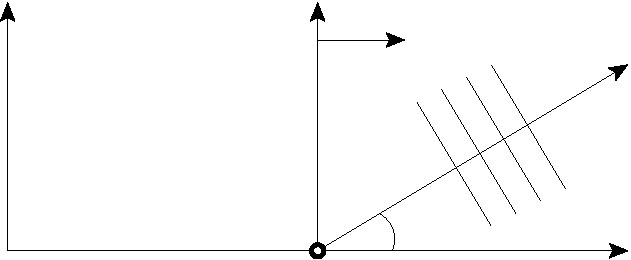
\includegraphics[scale=.6]{%
src/images/lbk-graphics/rel-dplr-efct} };
\node at (-2.9,.2) {\small$S$} ;
\node at (0.48,.2) {\small  $S^\bst(t)$} ;
\node at (0,-1.5) {\small  $P$} ;
\node at (3,.9) [right]{\small  $\vec{\gkk}$} ;
\node at (1,1.15){\small  $\vec{u}(t)$} ;
\node at (1,-1){\small  $\gka$} ;
\node at (2.5,-1.5) [right]{\small  $X,\, X^\bst$} ;
\node at (-3.1,1.5){\small  $Y$} ;
\node at (0.15,1.5){\small  $Y^\bst$} ;
\end{tikzpicture}
\end{center}
\caption{The relativistic Doppler effect}\label{fig8.1}
\end{figure}
To appreciate the Doppler effect further, we consider a 
(point) source of light $P$ which moves on the $x$-axis of 
the inertial frame $S$ with a velocity  $(u(t),\,0,\;0)$. 
Let $S^{\bst}(t)$ be the instantaneous rest frame of the 
moving source of light and let $ \gkw_\sfx{0}$ be the 
$S^{\bst}(t)$-frame frequency, i.e., the \textsl{proper 
frequency}, of the monochromatic plane light wave  
emitted by the source. Then, the first of the equations 
\eqref{ved.69x} relates the frequencies of the light wave 
in the two frames $S$ and $S^{\bst}(t)$ :
\begin{align}\label{ved.70x}
\gkw_\sfx{0} 
&=\gamma(\gkw -c \gkb\gkk_x) 
=\gamma(\gkw-\gkb c\gkk\cos\gka) = 
\gamma\gkw(1-\gkb\cos\gka),
\end{align}
where, now,  $\gkb=u(t)/c $, $\gamma=\sqrt{1- \gkb^2}$ and 
[see \figref{fig8.1}]
\begin{align}\label{ved.71x}
\vec{\gkk}= \gkk (\cos\gka, \sin\gka, 0) ,
\end{align}
is the wave-3-vector which we have taken to lie in the 
$x-y$ 
plane of the inertial frame $S$. in the $S$-frame. Also, we 
have replaced $c\gkk$ by  $\gkw$ in arriving at the last 
step in Eqn.\eqref{ved.70x}.

The final formula is obtained by rearranging 
\eqref{ved.70x} 
as
\begin{align}\label{ved.72x}
\gkw= \frac{\gkw_\sfx{0}\sqrt{1-\gkb^2}}
{(1 - \gkb\cos\gka)}\,.
\end{align}
We recall that, above,  we discussed the following  
situation. A monochromatic plane polarized light wave of 
\textsl{proper} or, \textsl{true} frequency $\gkw_0$, is 
radiated by a point source of light $P$ which moves with 
the 
3-velocity $\vec{u}(t)$, at the instant of time $t$, with 
respect to the inertial frame $S$. Furthermore, we assume 
that $P$ is radiating  monochromatic plane polarized 
light wave of \textsl{proper} or, \textsl{true} frequency 
$\gkw$. As observed from the inertial frame $S$, this light 
wave is observed, again, to be a  monochromatic, plane 
polarised wave, but both its  frequency $\gkw$ in $S$, 
as well as its direction of travel $\hat{\gkk}$ in $S$, 
would be different from the corresponding 
$S^\bst$-frame  values $\gkw_0$ and $\hat{\gkk}'$.  
Formula Eqn.\eqref{ved.72x}, called the 
\textsl{relativistic 
Doppler formula}, describes how the \textsl{relative 
frequency} $\gkw$ is related to  the \textsl{proper 
frequency} $\gkw_0$. The change in the direction of travel 
$\hat{\gkk}$ has already been discussed in \S~6.5 under 
aberration of light.

It is also useful to rewrite it in terms of the wavelength 
as follows:
\begin{align} \label{ved.73x}
\lambda_e&=\veca\lambda_\sfx{\,\,0}\frac{
\big(1-(v/c)\cos\theta\big)}
{\sqrt{1-v^2/c^2}}.
\end{align}
In passing, we note the some special cases of  
\eqref{ved.72x}:
\hbf{Case~1}
Setting $\gka =0 $ in \eqref{ved.72x}: We have
\begin{align}\label{ved.74x}
\gkw= \frac{\gkw_\sfx{0}
\sqrt{1-\gkb^2}} {(1 -\gkb)}= \gkw_\sfx{0}
\sqrt{\frac{1+\gkb}{1 -\gkb}}> \gkw_\sfx{0},
\end{align}
which gives the Doppler shift when {the source of light
moves towards the light wave} along the $x$-axis of 
$S$.

\hbf{Case~2}
Similarly, taking $\gka =\pi$, which corresponds to 
the 
case 
of the {source of light moving away from light wave} 
along 
the $x$-axis of $S$, we get
\begin{align}\label{ved.75x}
\gkw= \frac{\gkw_\sfx{0}\sqrt{1-\gkb^2}}
{(1+\gkb)}= \gkw_\sfx{0}\sqrt{\frac{1-\gkb}
{1 +\gkb}}<\gkw_\sfx{0}.
\end{align}

\hbf{3. The non-relativistic Doppler shift formula}
If the source of light moves very slowly compared to 
$c$, 
and the angle $\gka $ is not equal to $\pi/2 $, we may 
approximate the above formula by retaining only terms 
linear 
in $\gkb $ and we get
\begin{align}\label{ved.76x}
\gkw\approx
\gkw_\sfx{0}(1 +\gkb \cos\gka),
\end{align}
which is the familiar formula 
giving the \textsl{non-relativistic Doppler shift}.
\hbf{4. The transverse Doppler effect}
Setting  $\gka=\pi/2$ in \eqref{ved.72x}, we get
\begin{equation}\label{ved.77x}
\gkw=\gkw_\sfx{0}\sqrt{1-\gkb^2}\approx
\gkw_\sfx{0}\left(1-\gkb^2/2 \right),
\end{equation}
which is a \textsl{purely relativistic effect} 
corresponding 
to a frequency shift when the source of light and the 
light 
wave move at right angles to each other.

\exm{In a high precision experiment that uses  
Mossbauer 
effect, the emitter and absorber of photons are 
attached to 
the rim  of a centrifuge at points separated by an 
angle 
$\gka$ as measured in the (inertial) lab-frame.  
Calculate the red-shift and show that, for all angles 
$\gka$, resonance is not destroyed when the centrifuge 
rotates.[See Misner,Thorne  and Wheeler, p. 63-4; for 
an 
alternative calculation.]}

\soln If $\lambda_e$ and $\lambda_a$ are the 
wavelengths of
the emitted and absorbed photons, then
\begin{align}
 z=\frac{\lambda_a - \lambda_e}{\lambda_e}
\end{align}
is the standard measure of the red-shift which we 
shall 
calculate now using the Doppler formula 
Eqn.\eqref{ved.73x}. 

\begin{figure}[H]
\begin{center}
\begin{tikzpicture}
%   \draw[help lines,step=.25,red] (-4,-4) grid (5,5) ;
%   \foreach \y in {-4,-3.5,...,5}
%     \draw (-4.2,\y) node[left]{\tiny\y} ;
%   \foreach \x in {-4,-3.5,...,5}
%     \draw (\x,-4.2) node[below]{\tiny\x} ;
\node at (0,0)
{\includegraphics[scale=1]%
{src/images/lbk-graphics/dop-centrifuge1.pdf}};
\node at  (.2,.9) {\small  Photon};
\node at (-2.5,-0.28) 
{\small  $B$};
\node at (3.6,1.25) {\small  $A$};
\node at (.9,-.7) {\small  $O$};
\node at (-.5,-.7) {\small  $r$};
\node at (2.25,0.1) {\small  $r$};
\node at (.7,-.2) {\small  $\gka$};
\node at (2.9,1.25) [left]{\small  $\gkq$};
\node at (-2.5,-1.25){\small  $\phi$};
\node at (-.5,-.27) {\small  $\varepsilon$};
\node at (1.7,.35){\small  $\varepsilon$};
\node at (-2.4,-2.9){\small  $\vec{v}_\sfx{B}$};
\node at (2.4,3.0){\small  $\vec{v}_\sfx{A}$};
\end{tikzpicture}
\end{center}
\caption{}
\end{figure}

In the lab-frame (see Figure~8.2), when the centrifuge 
is 
not  rotating, let  $ r $ be the radius of (the rim 
of) 
the centrifuge and $\gkw $ be its angular rotation 
frequency. Let a  Mossabauer pair of atoms be fixed to 
the rim of the centrifuge at positions making an 
anglke 
$\gka $ at the axis of the centrifuge. A photon of 
proper 
wavelength $\lambda_0 $ emitted by one of the atoms is 
resonantly absorbed by the other when the centrifuge 
is 
rotating.

When the centrifuge rotates, a photon that leaves the 
emitter  atom, say, at $A$, arrives at the  absorber 
atom 
(see Figure~8.2) when it is at  $B$. Now, because the 
emitter and absorber are not at rest relative to one 
another, because of Doppler effect, {a photon emitted 
at 
$A$ 
is not resonantly absorbed at $B$}. The experiment 
consists 
of adjusting the rotation frequency $\gkw$ of the 
centrifuge 
in the lab-frame such that resonance is 
re-established. 
When 
that happens, let $\lambda_0$,   $\lambda_e$ and 
$\lambda_a$ 
be the photon's proper-wavelength, the lab-frame 
wavelength 
when it is emitted, and the lab-frame wavelength when 
it is 
resonantly absorbed. Further, let $S_A$ and $S_B$ be 
the 
instantaneous (inertial) rest-frames of the source-atom 
and 
the absorber-atom at the instants $t_A$ and $t_B$ in 
the 
lab-frame when they are at $A$ and $B$. Then, the 
lab-frame 
wavelength of the photon when it is emitted at $A$ is 
related to its proper wavelength $\lambda_\sfx{\,\,0}$ 
by 
Eqn.\eqref{ved.73x}
\begin{align}\label{ved.71}
\lambda_e&=\frac{\lambda_\sfx{\,\,0}
\big(1-(v/c)\cos\theta\big)}
{\sqrt{1-v^2/c^2}}=\frac{\veca\lambda_\sfx{\,\,0}
\big(1-(r\gkw/c)\cos\theta\big)}{(1-r^2\gkw^2/c^2)}.
\end{align}
Here $\theta$ is the angle between $\vec{v}_\sfx{A}$ 
and the direction of travel of the wave at $A$ and we 
have written 
$|v_\sfx{A}|=r\gkw$.

The photon which leaves $A$ travels in a straight line
and   reaches  $B$ at which it's wavelength is
\begin{align}\label{ved.72}
\lambda_a=\frac{\veca\lambda_\sfx{\,0}
[ 1-(r\gkw/c)\cos\phi]}{(1-r^2\gkw^2/c^2)}.
\end{align}
From Fig.~8.2, we note that  $\theta = 
\pi/2-\varepsilon$ 
and   $\phi = \pi-(\pi/2+\varepsilon) = \theta$. Also, 
from the triangle $OAB$, we have $(\pi/2-\varepsilon) 
=\gka/2$ so that $\cos\theta=\cos\phi=\cos(\gka/2)$. 
Thus,
\begin{align}\label{ved.73}
\lambda_a =\lambda_e=\frac{\veca\lambda_\sfx{\,\,0}
[1-(r\gkw/c)\cos(\gka/2)]}
{(1-r^2\gkw^2/c^2)}\Rightarrow z=0,
\end{align}
for all angles $\gka$. In other words, \textsl{resonance is 
not destroyed when the centrifuge is set into rotation.}

\section*{Exercises}
\exise For an electrostatic field,  show that  
the equation \eqref{ved.20x} reduces to the Coulomb law 
\begin{align}
\nabla^2 \varphi=-\frac{\rho}{\epso}.
\end{align}
in the Coulomb gauge ($\pdv{\varphi}{t}=0, \vec{A}=0$).
\exise Directly verify the second relation in  
Eqn.\eqref{ved.45x} under an $x$-boost.


\begin{small}
\begin{quote}
\hbf{Reference}

[1] L.D.Landau and E.M.Lifshitz, {The Classical   Theory
of Fields}, Cource of Theoretical Physics, Volume~2, Fourth 
Edition, Pergamon Press,   Oxford,1975

[2] J L Synge Relativity :  The Special Theory, North 
Holland Publishing Company, Amsterdam, 1972,  Chapter IX.

\end{quote}
\end{small}
